\documentclass[a4paper,14pt]{extarticle}

\usepackage[utf8]{inputenc}
\usepackage[russian]{babel}
\usepackage{amsmath}
\usepackage{amssymb}
\usepackage{MnSymbol}
\usepackage{wasysym}
\usepackage{mathtext}
\usepackage{mathenv}
\usepackage{listings}
\usepackage{color}
\usepackage{graphicx}
\usepackage{hyperref}
\usepackage{amssymb,amsfonts,amsmath,mathtext,cite,enumerate,float}
%\usepackage{algorithm}
\usepackage{float}
\usepackage[noend]{algpseudocode}
\usepackage[ruled,vlined]{algorithm2e}
\usepackage[a4paper, left=20mm, right=20mm, top=20mm, bottom=20mm]{geometry}
\usepackage{indentfirst}
\usepackage{epstopdf}

\DeclareGraphicsExtensions{.eps} 


\newtheorem{definition}{Определение}[section]
\newtheorem{remark}{Примечание}[subsection]
\newtheorem{suggest}[remark]{Соглашение}
\newtheorem{claim}[remark]{Утверждение}
\newtheorem{lemma}[remark]{Лемма}
\newtheorem{theorem}{Теорема}
\newtheorem{conseq}{Следствие}[theorem]
\newenvironment{Proof} 
{\par\noindent{\bf Доказательство.}} 
{\hfill$\blacksquare$}

\newenvironment{rusalgorithm}[1][htb]
{\renewcommand{\algorithmcfname}{Алгоритм}
\begin{algorithm}[#1]
}{\end{algorithm}}



\definecolor{dkgreen}{rgb}{0,0.6,0}
\definecolor{gray}{rgb}{0.5,0.5,0.5}
\definecolor{mauve}{rgb}{0.58,0,0.82}

\lstset{frame=tb,
language=Java,
aboveskip=3mm,
belowskip=3mm,
showstringspaces=false,
columns=flexible,
basicstyle={\small\ttfamily},
numbers=none,
numberstyle=\tiny\color{gray},
keywordstyle=\color{blue},
commentstyle=\color{dkgreen},
stringstyle=\color{mauve},
breaklines=true,
breakatwhitespace=true
tabsize=3
}

\renewcommand{\baselinestretch}{1.5}
\renewcommand{\leq}{\leqslant}
\renewcommand{\geq}{\geqslant}
\renewcommand{\phi}{\varphi}

\DeclareMathOperator{\Supp}{Supp}

\newcommand{\norm}{\mathop{\mathsf{norm}}\limits}
\newcommand{\sparse}{\mathop{\mathsf{sparse}}\limits}
\newcommand{\argmin}{\mathop{\mathsf{argmin}}\limits}
\newcommand{\argmax}{\mathop{\mathsf{argmax}}\limits}

\begin{document}
\begin{titlepage}

\begin{center}

«МОСКОВСКИЙ ФИЗИКО-ТЕХНИЧЕСКИЙ ИНСТИТУТ \\
(ГОСУДАРСТВЕННЫЙ УНИВЕРСИТЕТ)»\\[12em]

Департамент философии\\[1em]


{РЕФЕРАТ ПО ИСТОРИИ НАУКИ}\\[1em]
\textbf{\large История и развитие статистического анализа текстов}\\[6em]

\begin{minipage}{\textwidth}
\begin{flushright}
Аспирант --- Ирхин~И.~А
\end{flushright}
\end{minipage}\\[1em]

\begin{minipage}{\textwidth}
\begin{flushright}
Научный руководитель --- \underline{\hspace*{2.5cm}} Воронцов К.В.
\end{flushright}
\end{minipage}\\[1em]

\begin{minipage}{\textwidth}
\begin{flushright}
Преподаватель департамента философии --- Храмов О.С.
\end{flushright}
\end{minipage}\\[1em]
\vfill
{\normalsize Москва 2017}
\end{center}
\end{titlepage}

\tableofcontents
\newpage
\renewcommand{\baselinestretch}{1.5}
\section{Введение}


Анализ текстов --- это направление в машинном обучении, целью которого является получение информации из больших коллекций текстовых документов. Согласно Википедии: <<Ключевыми группами задач анализа текстов являются: категоризация текстов, извлечение информации и информационный поиск, обработка изменений в коллекциях текстов, а также разработка средств представления информации для пользователя.>>

Расшифруем упомянутые в этой фразе задачи. Категоризацией документов называют следующую задачу: имеется набор документов, требуется отнести каждый документ к одной или нескольким группам (обычно их называют классами или кластерами). Задача категоризации может решаться как при участии человека, так и без него. В первом случае сначала человек сам присваивает классы какой-то части документов, а затем использует методы машинного обучения, чтобы построить модель, которая будет экстраполировать назначенные человеком классы на произвольные документы. В машинном обучении такие задачи называют задачами обучения с учителем (этой терминологией мы будем пользоваться в дальнейшем). Во втором случае алгоритм должен сам выделить документы похожие друг на друга в отдельные группы. Такие задачи называют обучением без учителя. Также отдельного упоминания заслуживает задача информационного поиска. Если очень сильно упрощать, то её можно сформулировать так: поиск информативных (релевантных) объектов по заданному запросу в заранее известном множестве.

Анализ текстов широко применяется для решения прикладных задач во многих отраслях, в которых работают с большими объёмами данных. Дело в том, что большая часть информации, релевантной для бизнеса, находится в неструктурированном виде, например в виде сплошного текста. Методы анализа текстов позволяют извлечь важные закономерности, а также, что даже более важно, структурировать их. При этом для применения алгоритмов, как правило, не требуется вовлечение человека в процесс, большая часть решений принимается исключительно на основании каких-то статистических правил (хотя существуют подходы, позволяющие объединять статистические закономерности с дополнительными априорными знаниями людей о природе данных). Таким образом, применение техник анализа текстов, зачастую даёт конкурентное преимущество, что способствует их массовому применению в наши дни и, как следствие, популяризации этой области науки.

Вот несколько ярких приложений анализа текстов:
\begin{itemize}
\item Безопасность ПО. Так как код программы тоже является по сути текстом, то на его основании можно принимать решения о том, является ли вредоносной программа или нет. Также идеи методов анализа текстов можно встретить в криптографии.
\item Биомедицина и биоинформатика. Различные гены можно представить в виде текстовых последовательностей, что позволяет по иному взглянуть на задачи данной области. Также есть острая необходимость в улучшенном поисковике только по медицинским терминам.
\item Маркетинг. В последнее время популярность набирают различные вопросно-ответные системы, например, в банках, интернет магазинах и т.п. Также анализ текстов используется в прогнозировании поведения пользователей.
\item Создание искусственного интеллекта.
\end{itemize}

В данном реферате выделить две больших части. В первой будут описаны основные методы и задачи анализа текстов. Таким образом, будет построена некоторая картина мира, сложившаяся в области. К сожалению, формат реферата не позволяет охватить все тонкости развития данной науки, поэтому упор будет сделан на те аспекты, которые наиболее связаны с машинным обучением и тем, которые на взгляд автора наиболее важны с точки зрения истории развития области. Вторая часть будет посвящена так называемому тематическому моделированию. Коротко говоря, тематическая модель коллекции текстовых документов определяет к каким темам относится каждый документ и какие слова образуют каждую тему. Эта тема выбрана постольку, поскольку она непосредственно связана с диссертационной работой автора. 


\section{Общая история}
Прежде чем мы перейдём к непосредственному разбору методов и задач анализа текстов и истории их развития, хочется рассказать краткую историю развития области с целью создания целостной представления во времени.
Трудно определить момент возникновения науки под названием <<Анализ текстов>>. Уже в конце 50-ых годов появлялись некоторые статьи, которые оперировали и отмечали те идеи и подходы, которые используются в современности. Например, в 1957 году были в статье Luhn и Hans Peter. `A Statistical Approach to Mechanized Encoding and Searching of Literary Information' были озвучены идеи использования различных статистик для отражения информативности документов. Но поскольку в этот период ещё не существовало необходимых вычислительных мощностей, дальше формулирования концепций до середины 80-ых не заходило. Хотя, начиная с 60-ых появляются исследования, в которых производится какая-то простая статистическая аналитика текстов, например, подсчёт частоты встречаемости букв (пар, троек буквы и т.п.) или слов в различных языках. Например в 1965 году Mayzner и Tressel опубликовали `Tables of single-letter and digram frequency counts for various word-length and letter-position combinations'.

Тем не менее период с 50-ых до 80-ых весьма важен для развития анализа текстов. Дело в том, что в это время активно развивался математический аппарат, который станет активно использоваться в будущем, а также позволит формализовать и довести до строгих формул предложенные концепции и подходы. Особенную роль сыграло развитие теории информации. В качестве простого примера можно привести статью Kullback и Leibler 1951 года `On information and sufficiency', в которой была предложена функция, по которой можно измерять взаимную информацию между двумя распределениями. Эту функцию назовут в честь авторов дивергенцией Кульбака-Лейблера и она станет если не самой важной, то одной из самых важных функций расстояний между вероятностными распределениями. Другим хорошим примером может служить развитие Hidden Markov Model (HMM), которые, как оказалось, неплохо подходят для описания появления слов в предложениях.

В середине 80-ых годов стали появляться статьи, которые предлагали уже конкретные подходы и формализации, и, что более важно, какие-то реальные эксперименты по их применению. В основном они сводились к предложению различных полезных статистик, которые могут быть информативны для определения свойств текста. Например, в это время появилась идея tf–idf, которую мы более подробно опишем в следующих разделах.

В 90-ых годах становятся популярными матричные разложения, в этот период было опубликовано множество статей на эту тему. Особенно популярными были неотрицательные матричные разложения, которые лучше отражали природу текста. Сильное влияние на популяризацию матричных разложений сыграл Netflix Prize. Netflix --- компания, специализирующая на предоставлении онлайн фильмов. В 2006 году они начали конкурс, в котором нужно было научиться предсказывать оценки, которые поставят пользователи тем или иным фильмам. Оказалось, что это задача напрямую связана с задачей матричного разложения. Но самый главный фактор в этой истории --- победитель получал 1 млн. долларов. Поэтому наука очень сильно продвинулась в матричных разложениях, потому что, как говорил один из преподавателей автора: << Одно дело наука ради науки, а другое наука ради миллиона долларов>>.

Крайне важным историческим моментом является статья Hofmann и Thomas 1999 года `Probabilistic Latent Semantic Indexing', в которой был предложен алгоритм Probabilistic Latent Semantic Analysis (PLSA). В этой статье была предложена вероятностная модель текста, которая позволяла происзводить кластеризацию документов и слов. Эта статья положила начало тематическому моделированию. Конечно же, предложенный метод имел множество недостатков, тем не менее новый подход и модель, которые были предложены стала основой большого множества статей. Более подробно про тематическое моделирование будет рассказано в соответствующей главе. Одним из главных минусов подхода матричных разложений было то, что они никак не учитывали порядок слов в документах, рассматривая их как некоторый `мешок слов' (то есть было важно сколько раз слово встретилось в документе, но не где именно). Поэтому их старались скрещивать с HMM, которые позволяли этот порядок учитывать.

Если не вдаваться в подробности, то период с начала 90-ых до конца 00-ых можно охарактеризовать следующим образом. Во-первых, с развитием информационных и вычислительных технологий стали появляться новые задачи в новых отраслях и новые текстовые данные, причём в больших объёмах, на которых можно было проверять новые подходы и методы. В основном это всё были задачи категоризации текстов. Если выразиться просторечно, то анализ текстов `пошёл в массы'. Во-вторых совершенствовались уже предложенные идеи и подходы. Например, в матричных разложениях пытались учитывать дополнительную информацию о природе текста (его авторов, источник текста, время издания и т.д.), усложняли вероятностную модель текста и многое другое.

Но в начале 10-ых произошло событие, которое изменило всё. Оно произошло немного в другой области машинного обучения, но затронуло практически все его направления, а именно в области нейросетей. Сделаем небольшую историческую ремарку. Согласно Википедии: <<Искусственная нейронная сеть --- математическая модель, а также её программное или аппаратное воплощение, построенная по принципу организации и функционирования биологических нейронных сетей --- сетей нервных клеток живого организма>>. Нейронные сети были известны науке относительно давно (по современным меркам). Уже в конце 80-ых были статьи, которые описывали данную математическую модель. Стоит отметить, что качество предсказаний у данной модели было весьма высоким. Но, к сожалению, у неё было две больших проблемы: во-первых, для обучения требовалось очень много данных, а во-вторых, на момент создания не было известно эффективного способа обучать эти модели. Предложенные градиентные методы оптимизации работали невозможно долго, и потому развитие этой области приостановилось. Но на рубеже веков был придуман новый метод --- Backpropagation, который позволил существенно сократить временные затраты. А к концу 00-ых была разработана удобная инфраструктура для сбора данных и последующего обучения нейросетей на этих данных. Как результат, в начале 10-ых произошёл мощный подъём популярности этой модели и можно смело сказать, что на текущий момент это самый популярный и state-of-the-art метод машинного обучения.

Под влияние вышеописанного бума попала и область анализа текстов. Если выделять самые главные применения нейросетей, то наиболее важными являются следующие два пункта: во-первых, это появление word2vec-алгоритмов (когда хочется научиться представлять слово в виде вектора таким образом, что сумма и разность векторов будет иметь какой-то физический смысл, знаковой статьёй тут является статья 2013 года от Mikolov и Tomas `Efficient Estimation of Word Representations in Vector Space'), а во вторых это появление рекуррентных нейронных сетей. Обе идеи довольно сложные и будут изложены в соответствующих разделах.

Это все основные исторические моменты (по мнению автора), которые можно выделить в истории развития текстов. Теперь мы перейдём к более детальному разбору упомянутых выше подходов. 
\subsection{Задача категоризации текстов}
Задачу машинного обучения с учителем можно сформулировать следующим образом. Существует множество объектов $X$, и множество ответов $Y$, а также какой-то набор данных $(x_i, y_i)$, где $x_i \in X$, $y_i \in Y$ при этом предполагается, что существует некоорая зависимость между этими двумя множествами, то есть существует некая функция $a \colon X \to Y$, такая, что $a(x_i) = y_i$. Цель метода машинного обучения восстановить эту зависимость по имеющимся данным. Конечно же, абсолютно точно восстановить такую зависимость нельзя, поэтому обычно ищется наиболее хороший алгоритм по какой-то заранее зафиксированной метрике качества предсказаний алгоритма. Например, известный метод МНК: даны $x_i,~y_i$, требуется найти такие $a$ и $b$, что $\sum_i (y_i - a x_i - b)^2 \to min$.Но в отличие от этой большинство задач машинного обучения не решаются аналитически, приходится использовать сложные методы оптимизации, такие как градиентные методы или генетические алгоритмы и многие другие.

Но вернёмся к анализу текстов. Важным моментом в решении задачи машинного обучения является построение признаков объекта. Как правило, объект имеет сложную структуру, которую нельзя просто так формализовать (как правило мы хотим получить вектор чисел --- признаковое описание объекта). В анализе текстов это как нельзя важная проблема --- текст это большой и сложный объект, а нам нужно придумать какие-то его признаки, чтобы их было не слишком много, но при этом они хорошо описывали суть текста.

Простейшим вариантом является подход `bag-of-words', когда описанием текста является просто список частот всех входящих в него слов:
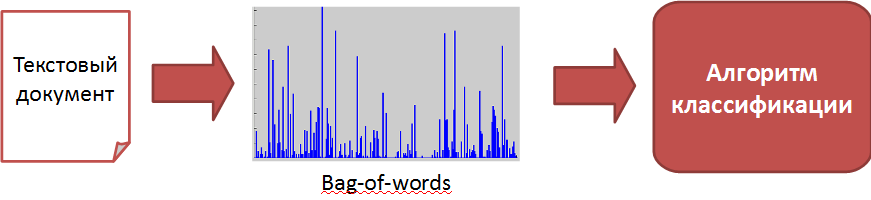
\includegraphics[width=1.0\linewidth]{bag_of_words.png}

Этот подход начинали практиковать уже в конце 70-ых, однако у него был ряд минусов. Не будем вдаваться в подробности, уточним только основной из них, признаки никак не учитывали разную важность слов, например, артикли в английском языке не особо информативны, потому что практически везде встречаются и информация о их наличии становится бесполезной. Эта проблема была частично решена за счёт tf-idf подхода, который был упомянут ранее.

Пусть имеется коллекция документов $D$, каждый документ $d$ состоит из терминов $t$, тогда 
\[
tfidf(t, d, D) = tf(t, d) idf(t, D),
\]
где $tf(t, d)$ --- term frequency, частота термина $t$ в документе $d$, а $idf(t, D)$ --- inversed document frequency, минус логарифм доли документов, где встречается термин $t$. Таким образом, частые слова начинали иметь меньший вес, что положительно сказывалось на качестве обучаемых моделей. На сегодняшний день существует масса вариаций того, как можно считать $tf$ и $idf$, однако, общая идея данных величин осталась неизменной и была заложена ещё в середине 80-ых годов.

К сожалению, в таком подходе количество признаков текста --- количество различных слов коллекции (в документе для каждого слова нужно знать какое-то число, которое обычно нулевое), что порой слишком много. В этом случае обычно применяют алгоритмы понижения размерности данных, в основном это алгоритмы матричных разложений.
\subsection{Матричные разложения}
В чём заключается задача матричного разложения? Пусть имеется какая-то матрица $N$ размера $W \times D$, где $W$ и $D$ достаточно велики. Требуется найти матрицу $\Phi$ размера $W \times T$ и матрица $\Theta$ размера $T \times D$, где $T$ достаточно малы, такие что $N \approx \Phi \Theta$. Формализация того, что именно означает приблизительно равно в этой записи, определяет различные методы разложений.

Например, если задача ставится как $||\Phi \Theta - N||^2 \to \min$, то это будет задача Singular Value Decomposition (SVD), которая была известна ещё в первой половине 20го века, но в анализе текстов стала использоваться в середине 90-ых годов. Если добавить ограничение неотрицательности всех элементов на матрицы $\Phi$ и $\Theta$, то будет получена задача Nonnegative Matrix Factorization, которая тоже неплохо себя зарекомендовала в тот же временной период. Если минимизировать дивергенцию Кульбака-Лейблера между столбцами $N$ и $\Phi\Theta$, то будет получена задача тематического моделирования и алгоритм Probabilistic Latent Semantic Analysis (PLSA).

Непосредственных применений матричных разложений очень много. Это и упрощение признакого описания слов и документов (строчки матрицы $\Phi$ и столбцы матрицы $\Theta$ соответсвенно), и поиск похожих сущностей (сводится к поиску близких векторов), и автоматическая разметка документов (на основании векторов-описаний слов) и многое другое.

Хочется ещё раз рассказать о Netflix Prize. Как уже говорилось, этой компанией был организован конкурс по прогнозированию оценок фильмов пользователями. Пусть $U$ --- число пользователей, $V$ --- число видео, $T$ --- внутренний параметр. Тогда имеется матрица $R$ размера $U \times V$, но некоторые оценки скрыты. Качество алгоритма измерялось как среднеквадратичное отклонение между предсказанными оценками и реальными. Пусть матрица $\Phi$ размера $U \times T$ содержит в строках скрытые вектора размера $T$, описывающие предпочтения пользователей, а матрица $\Theta$ размера $T \times V$ в стобцах вектора-описания видео. Тогда требуется построить разложение, решающее задачу $||\Phi \Theta - R||^2 \to \min$. Небольшая трагедия состоит в том, что была выбрана квадратичная функция. Дело в том, что она очень легко считается, но никак не связана с природой задачи (например, очень часто в прикладных задачах нужно считать расстояния между распределениями, а квадратичная метрика очень плохо для этого подходит). Тем не менее, в конкурсе была назначена именно эта функция. Как результат, были изобретены новые методы и подходы к матричным разложениям, которые давали существенный прирост качества моделей, но именно по квадратичной функции измерения ошибки. Этот конкурс хорошо показывает, как однажды принятое неудачное решение может сильно перенаправить научное течение в не то русло на многие годы.

\subsection{HMM}
Важную роль в развитии анализа текстов сыграли hidden markov models (HMM). Неформально их можно объяснить следующим образом. Есть какие-то наблюдаемые величины $y_t$, $t = 0..T$. Предполагается, что появление того или иного значения $y_t$ обусловлено какой-то внутренней, скрытой и ненаблюдаемой величиной $x_t$ (это смысл слова hidden в названии). Причём значение $x_{t+1}$ определяется исключительно значением $x_t$ (это смысл слова markov в названии).

\medskip

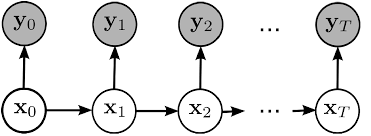
\includegraphics[width=1.0\linewidth]{hmm.png}

Приведём довольно простой пример. Вы пришли в казино и играете с крупье в подбрасывание монетки. У крупье есть две монетки: обычная и фальшивая, особенность фальшивой в том, что орел на ней выпадает с вероятностью $0.9$, а не $0.5$, как на обычной. В каждом раунде игры крупье решает какую монетку использовать по следующему правилу: с вероятностью $0.8$ оставляет ту же монетку, что и в прошлом раунде, а с вероятностью $0.2$ меняет. Таким образом, скрытой величиной здесь будет тип монетки, а наблюдаемой величиной --- результат броска.

Для HMM существует множество задач: найти наиболее вероятную цепочку внутренних состояний (решается при помощи алгоритма Витерби, первые упоминания которого можно найти в конце 90-ых годов); оценить связь между скрытым состоянием и наблюдаемым (это особо актуально, когда точные значения вероятностей не заданы, в отличие от приведённого примера)

В случае анализа текстов наблюдаемыми величинами являются слова, а скрытыми состояниями могут быть тематика слова или его часть речи. Такие работы были популярны в начале 00-ых. Также HMM используются для распознавания речи, в таком случае наблюдаются звуки, а скрытым состоянием является произносимое слово. Работы по данной тематике можно найти в основном, начиная с конца 00-ых годов.

В настоящее время популярны становятся графические модели. Идеологически они продолжают дело марковских цепей, но позволяют учитывать более сложные зависимости между наблюдаемыми и ненаблюдаемыми величинами (формально задаётся граф связей, отсюда и название метода).

Парралельно методу HMM развивался метод Conditional Random Fields (CRF). Чтобы объяснить их различие нужно сделать небольшую ремарку в сторону машинного обучения. При вероятностном подходе к решению этих задач, неопределенность в зависимости между X и Y моделируется введением совместного распределения на все переменные p(X, Y). Выделяют два вида вероятностных моделей: порождающие (generative) и дискриминативные (discriminative). При использовании порождающих моделей необходимо задать совместное распределение p(X, Y) на множестве
объектов, а в дискриминативных моделях условное распределение p(X|Y) на множестве значений скрытых переменных объекта. Генеративная модель, как правило, существенно сложнее устроена, но позволяет порождать новые объекты. А дискриминативная устроена проще, но и возможностей для использования даёт меньше, хотя для практики это обычно достаточно.

Если сильно упрощать, то CRF является дискриминативным аналогом HMM, в котором заменили совместное распределение величин условным:

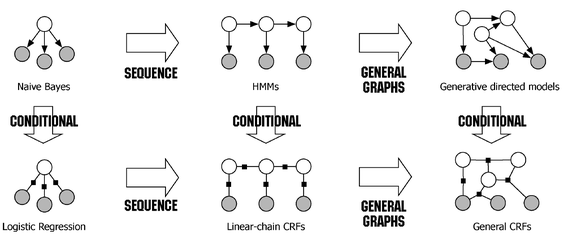
\includegraphics[width=1.0\linewidth]{hmm_crf.png}

Как и HMM линейные CRF сегодня практически не используются, предпочтение отдаётся обобщённым CRF, позволяющим учитывать произвольную графовую структуру. Что касается области применения CRF, то она примерно такая же как и у HMM. Разница лишь в том, как именно будет использоваться модель: если требуется генерировать речь или текст, то подходит только HMM, а для задач распознования подходят оба метода.
\subsection{Рекуррентные нейронные сети}
\subsubsection{Введение в нейронные сети}
Для начала объясним что такое нейронная сеть. Чтобы не вдаваться в математические подробности, приведём описание строения нейронной сети из Википедии: << Нейронные сети представляют собой систему соединённых и взаимодействующих между собой простых процессоров (искусственных нейронов). Такие процессоры обычно довольно просты (особенно в сравнении с процессорами, используемыми в персональных компьютерах). Каждый процессор подобной сети имеет дело только с сигналами, которые он периодически получает, и сигналами, которые он периодически посылает другим процессорам. И, тем не менее, будучи соединёнными в достаточно большую сеть с управляемым взаимодействием, такие по отдельности простые процессоры вместе способны выполнять довольно сложные задачи.>>

\medskip

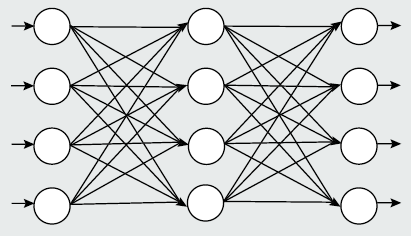
\includegraphics[width=1.0\linewidth]{neuronet.png}

Нейроны одного уровня называют слоем. Для нейрона необязательно быть связанным со всеми нейронами предыдущего слоя. Характер связей нейронов одного своя с предыдущим определяет тип слоя. На сегодняшний день известно множество типов слоёв: полносвязные, конволюционные, drop out, рекуррентные и многие другие. Совокупность всех слоёв и их типов и взаиморасположения определяет архитектуру нейронной сети.

Как говорилось в изложении общей истории, концепция первых нейронных сетей стала известна ещё в конце 70-ых годов, однако архитектура тех сетей была очень проста, наподобие той, что на картинке выше. Однако в конце 00-ых произошёл подъём этой области и архитектуры нейросетей очень сильно усложнились, количество слоёв сильно выросло. Например вот так выглядит архитектура нейросети Google 2014 года для распознавания изображений:

\medskip

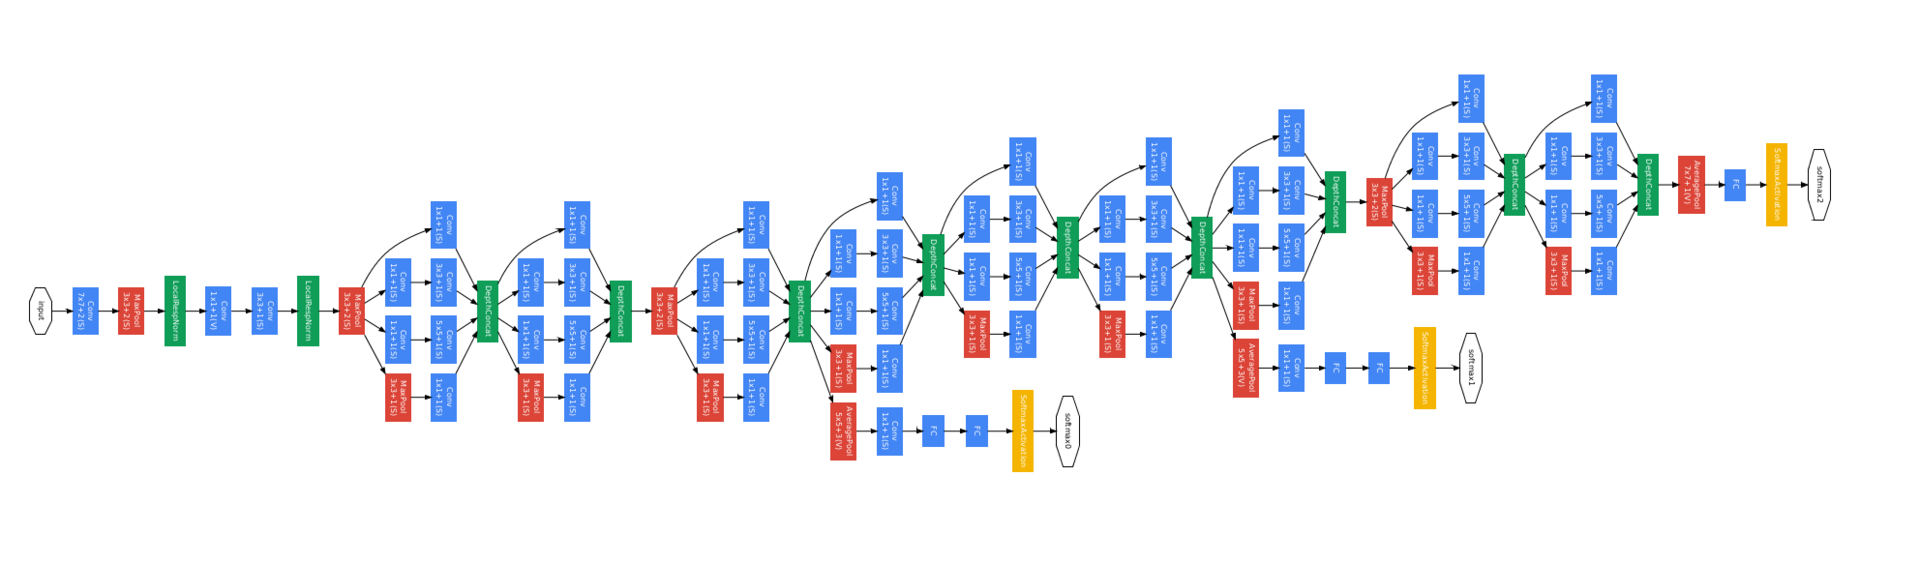
\includegraphics[width=1.0\linewidth]{net.png}

Из-за усложнения архитектур сильно выросло время обучения и количество необходимых для этого данных. Но отчасти благодаря этой проблеме люди обратили внимание на альтернативные способы вычислений. Большинство вычислений на современном компьютере происходит на процессоре (CPU), который специально спроектирован так, чтобы при повседневном использовании давать максимум производительности. Однако, обучение нейросети это далеко не повседневное использование CPU. Оно вовлекает множество перемножений матриц и других численных операций, которые, как оказалось, активно выполняются на видеокартах при отрисовке графики. Поэтому в конце 00-ых была разработана технология CUDA, которая позволяла использовать GPU в вычислениях. Наличие этой технологии оказало сильное влияния на воскрешения нейросетей. Современные нейросети могут обучаться порядка нескольких недель и это считается нормой. Хотя простые архитектуры способы обучаться и за несколько часов. 

\subsubsection{Рекуррентные нейронные сети}
При обучении нейронных сетей обычно использвуется метод стохастического градиента: берётся случайный объект, считается градиент, производится обновление параметров модели. Однако зачастую слова можно брать в определённом порядке, например, в порядке появления в тексте или в речи. Поэтому появилась идея использовать это в архитектуре нейронных сетей. Непосредственных формализаций весьма много, но принцип у всех довольно общий: нужно, чтобы слой получал свои значения с предыдущей итерации обучения. На картинке это будет выглядеть так:

\medskip

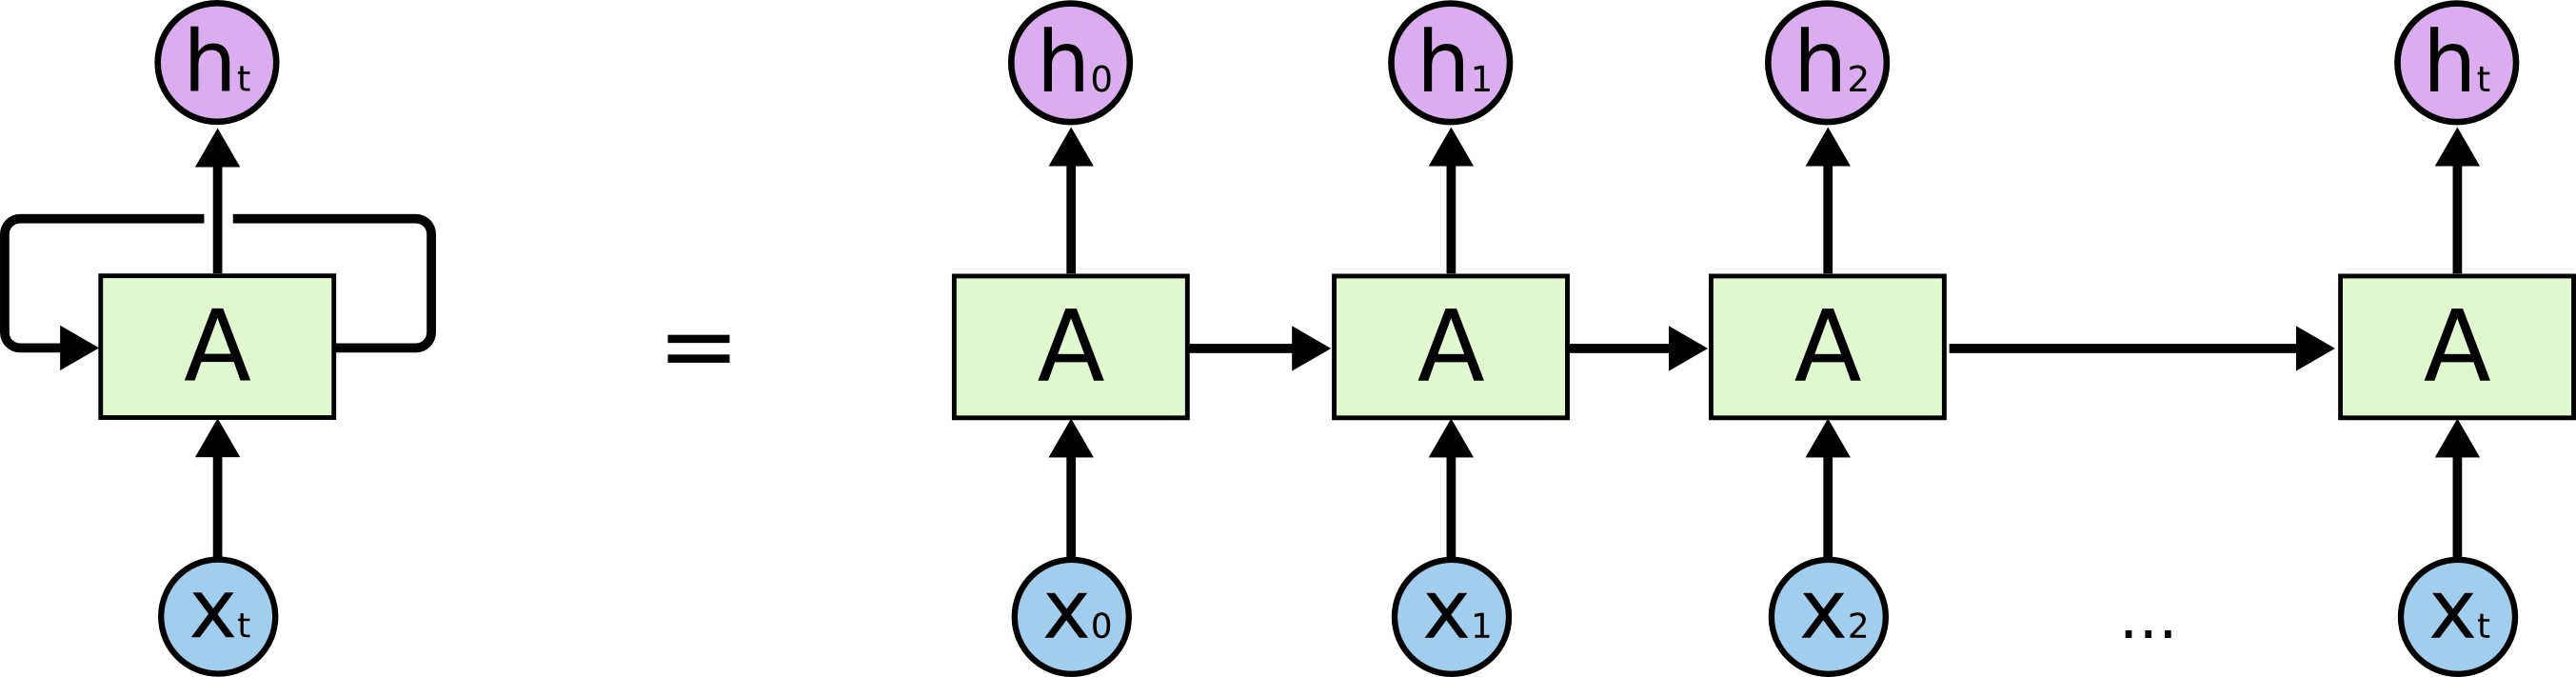
\includegraphics[width=1.0\linewidth]{rnn1.png}

Собственно, эта стрелка из слоя в себя и определяет рекуррентность. Как уже была сказано практически во всех задачах анализа текстов данные имеют последовательную структуру, поэтому применение RNN довольно перспективно. Нейронная сеть также позволяет комбинировать информацию от разных источников --- архитектура сети позволяет ей самой отобрать важные факторы для предсказаний.

\medskip

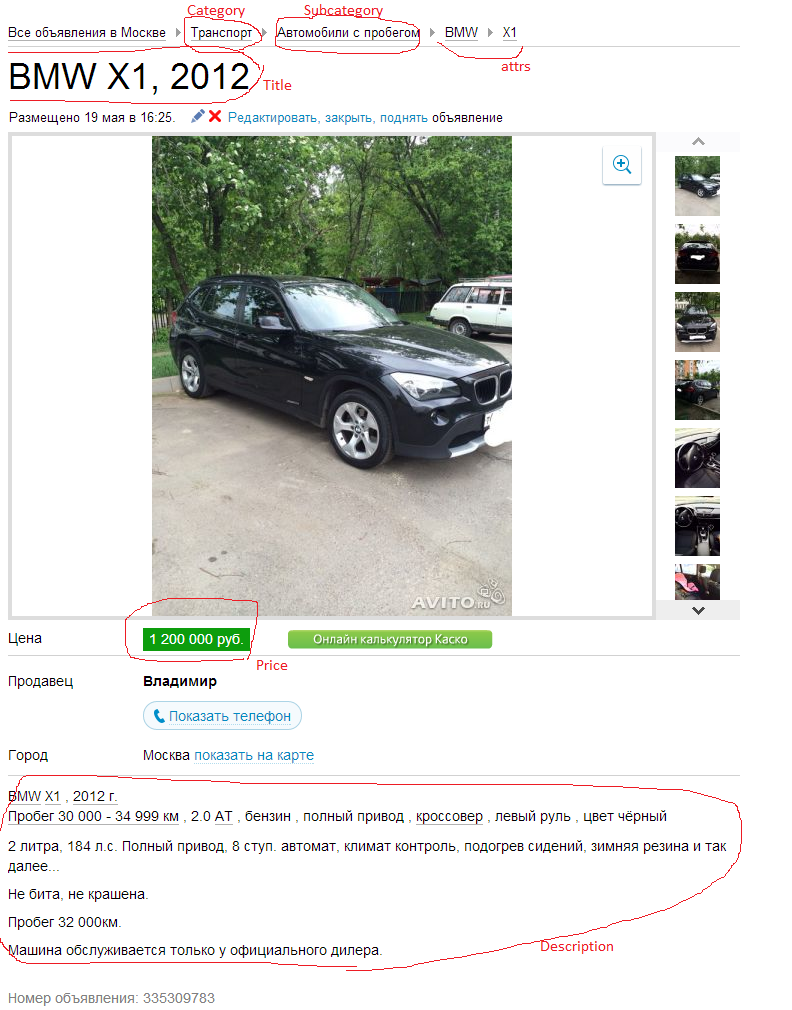
\includegraphics[width=0.4\linewidth]{rnn2.png}
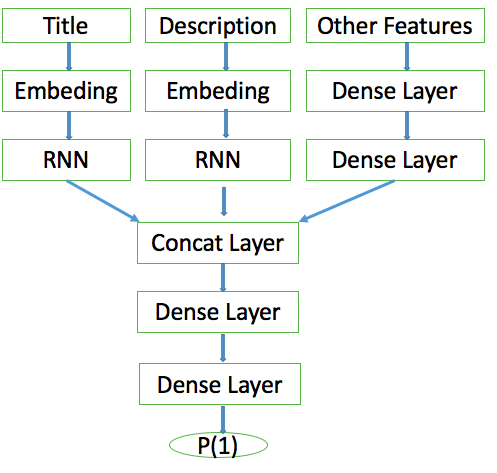
\includegraphics[width=0.4\linewidth]{rnn3.png}

\subsection{word2vec}
Последним из наиболее важных методов анализа текстов хочется выделить методы дистрибутивной семантики и алгоритма word2vec как некий венец творения данного направления. Основной идеей дистрибутивной семантики является следующее: смысл слова это набор контекстов, в которых оно встречается, то есть, если слова встречаются в одинаковых контекстах, то они похожи и наоборот.

Как обычно, приведём цитату из Википедии: <<Word2vec – программный инструмент анализа текстов, представляющий собой технологию, которая основана на векторном представлении слов. Этот инструмент был разработан группой исследователей Google в 2013 году. Работа этой технологии осуществляется следующим образом: word2vec принимает текстовый корпус в качестве входных данных и сопоставляет каждому слову вектор, выдавая координаты слов на выходе. Сначала он создает словарь, «обучаясь» на входных текстовых данных, а затем вычисляет векторное представление слов. Векторное представление основывается на контекстной близости: слова, имеющие схожий смысл и встречающиеся в тексте рядом с одинаковыми словами, в векторном представлении будут иметь близкие координаты векторов-слов. Полученные векторы-слова могут быть использованы для обработки естественного языка и машинного обучения. >>

По факту word2vec является простой нейросетью, которая, как оказалось, даёт очень хороший результат:

\medskip

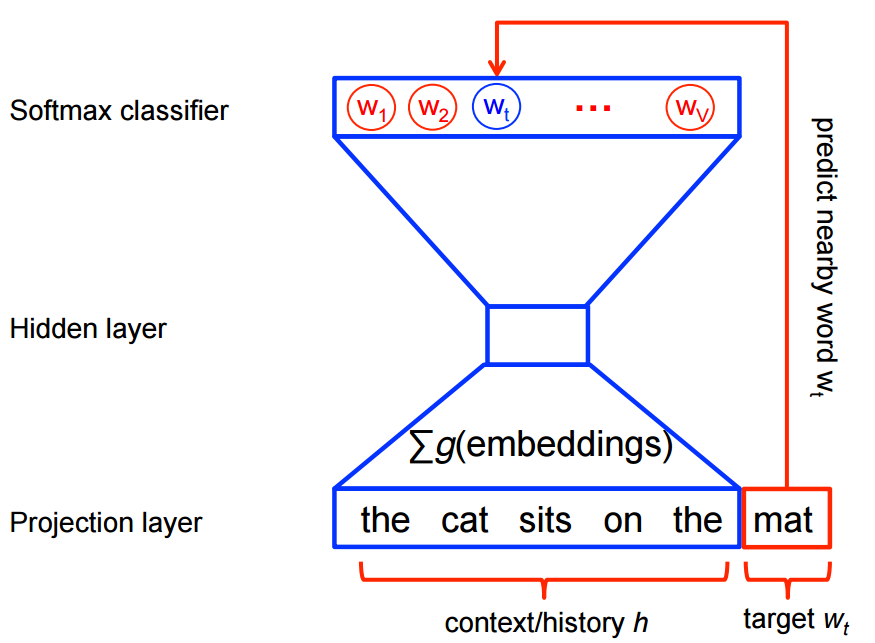
\includegraphics[width=1.0\linewidth]{word2vec.png}

На полученных словах можно ввести меру близости (обычно берут косинус угла между векторами). И тут становится заметно самое замечательное свойство word2vec:
\[
vec(\text{`king'}) - vec(\text{`man'}) + vec(\text{`woman'}) \approx vec(\text{`queen'})
\]
\[
vec(\text{`queen'}) - vec(\text{`king'}) + vec(\text{`kings'}) \approx vec(\text{`queens'})
\]

\medskip

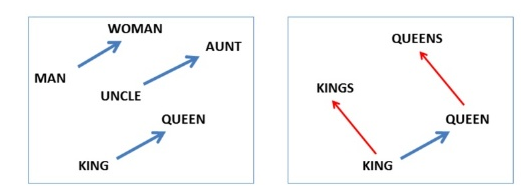
\includegraphics[width=1.0\linewidth]{word2vec_2.png}

Оказалось, что векторное вложение обладает свойством смыслового сложения и вычитания. Это оказалось крайне востребовано для области создания искусственного интеллекта: машина сможет <<понимать>> смысл слова, производя арифметические операции над векторами. Таким образом, за несколько лет (с 2013 года) этот метод обрёл гигантскую популярность и широко применяется в индустрии. Но он активно дорабатывается и совершенствуется: например, появились doc2vec и paragraph2vec, которые преобразуют к вектору, не слова, а целые документы или параграфы текста соответственно.
\section{История тематического моделирования}
История тематического моделирования прекрасно описана Воронцовым К. В. в 2014 году в Докладе РАН `Аддитивная регуляризация тематических моделей коллекций текстовых документов', в рамках которого был представлен новый одноимённый подход в тематическом моделировании.  В докладе довольно точно описаны другие работы и методы, коотрые они предлагали, поэтому практически полностью раздел является цитированием данного источника.

Для начала приведём напоминание того, что из себя представляет задача тематического моделирования:

<<Вероятностное тематическое моделирование ---
это современный мощный инструментарий статистического анализа текстов,
предназначенный для выявления латентных тем в коллекциях документов [Blei
2012]. Вероятностная тематическая модель (ВТМ) определяет тему как
совокупность слов, которые часто употребляются совместно в документах
коллекции. Например, в коллекциях научных публикаций темы могут
соответствовать явлениям, теориям, методам, при описании которых используется
устоявшаяся терминология. В коллекциях новостных сообщений темы могут
соответствовать событиям, странам, компаниям, персонам и т. д.
ВТМ осуществляет «мягкую» кластеризацию слов и документов по кластерам-
темам. «Мягкость» означает, что слово или документ могут относиться к
нескольким кластерам-темам с различными вероятностями. Тем самым выявляется
тематическая структура документов, а также решаются проблемы синонимии и
омонимии, возникающие при обычной «жёсткой» кластеризации. Синонимы, часто
употребляющиеся в схожих контекстах, с большой вероятностью попадают в одну
тему. Омонимы, употребляющиеся в разных контекстах, распределяются между
несколькими темами соответственно частоте их употребления.>>

\subsection{Методы тематического моделирования}
Текст взят из того же доклада РАН 2014 года: <<Вероятностный латентный семантический анализ (probabilistic latent semantic
analysis) PLSA [Hofmann 1999] и латентное размещение Дирихле (latent Dirichlet
allocation) LDA [Blei 2003] считаются стандартными методами вероятностного
тематического моделирования и часто используются в прикладных исследованиях.
В литературе описаны сотни их обобщений и модификаций [Daud 2010], имеются
доступные реализации. Несмотря на интенсивный поток исследований в этой
области, многие проблемы, в частности, проблемы неустойчивости и слабой
интерпретируемости тем, пока не имеют окончательного решения.
Интерпретируемость тем является плохо формализуемым требованием.
Предполагается, что, увидев список наиболее частотных слов и документов темы,
человек сможет понять, о чём эта тема, дать ей адекватное название, определить
более общие, более частные или близкие темы.

Интерпретируемость тем важна для
приложений тематического моделирования — информационного поиска,
категоризации, аннотирования, сегментации текстов. Интерпретируемость тем
позволяет систематизировать, визуализировать, объяснять результаты,
выдаваемые пользователю информационной системы.


Однако темы, найденные с помощью ВТМ, часто оказываются непонятными,
содержат слишком много слов, включают слова общей лексики, кажутся смесью
нескольких слабо связанных тем, оказываются слишком похожими на другие темы.
Более того, многократное обучение модели по одной и той же коллекции может
давать совершенно разные темы в зависимости от случайного начального
приближения. Исследователи либо мирятся с этими недостатками, не добиваясь
понятности латентных тем, либо отказываются от применения ВТМ, не находя
достойных альтернатив доступным реализациям PLSA и LDA.


Фундаментальная причина этих недостатков в том, что задача построения ВТМ
по коллекции документов имеет бесконечно много решений, лишь малая доля
которых интерпретируемы. Алгоритм оптимизации ВТМ выдаёт некоторое
произвольное решение из этого множества.

Задачи, решение которых не существует, не единственно или не устойчиво, в
математике принято называть некорректно поставленными (по Адамару). Известен
общий подход к их решению, называемый регуляризацией. Он заключается в том,
что для выбора наилучшего решения задаются дополнительные критерии
оптимальности, учитывающие специфические требования решаемой задачи и
называемые регуляризаторами. Если вводится несколько критериев, то задача
оптимизации становится многокритериальной. В данной работе рассматриваются
требования интерпретируемости и предлагается их формализация в виде набора из
четырёх регуляризаторов.

К сожалению, возможности гибкого введения регуляризаторов в PLSA и LDA не
предусмотрены ни в теории, ни в реализациях. Современные ВТМ основаны на
байесовском подходе, в котором комбинирование регуляризаторов вызывает
структурные изменения модели и наталкивается на значительные технические
трудности. Попытки построения многоцелевых ВТМ на основе LDA и генетических
алгоритмов [Khalifa 2013] представляются громоздкими и вычислительно
неэффективными. Большинство байесовских моделей, начиная с LDA, используют
в качестве основного регуляризатора априорное распределение Дирихле.
Это довольно сильное вероятностное допущение, которое не имеет убедительных
лингвистических обоснований, не улучшает интерпретируемость и устойчивость
модели, и затрудняет комбинирование регуляризаторов.

В данной работе для комбинирования регуляризаторов применяется новый
подход, альтернативный байесовскому — аддитивная регуляризация тематических
моделей, ARTM [Vorontsov 2014]. Он свободен от избыточных вероятностных
допущений, не требует введения распределений Дирихле и позволяет использовать
регуляризаторы, вообще не имеющие вероятностной интерпретации. Включение
ещё одного регуляризатора в модель выполняется «в одну строку» по готовым
формулам, намного проще, чем в байесовском подходе.

Предлагаемый подход к повышению интерпретируемости основан на
предположении, что если тема интерпретируема, то в ней имеется ядро —
множество характерных слов, являющихся терминами определённой предметной
области, которые с большой вероятностью употребляются в данной теме и
практически не употребляются в других темах. Отсюда вытекают требования
разреживания и повышения различности тем, переноса слов общей лексики в
отдельные «фоновые» темы, и удаления незначимых тем. В данной работе эти
требования формализуются с помощью комбинации четырёх регуляризаторов.
Большинство существующих методов оценивания интерпретируемости
основано на привлечении экспертов-асессоров. В исследовании [Newman, 2009]
экспертам предлагалось непосредственно оценивать полезность тем по
трёхбалльной шкале. В методе word intrusion [Chang 2009] для каждой найденной
темы составляется список из 10 наиболее частотных слов, в который внедряется
одно случайное слово. Тема считается интерпретируемой, если подавляющее
большинство экспертов правильно указывают лишнее слово. Экспертные подходы
необходимы на стадии исследований, но затрудняют создание полностью 
автоматических технологий построения ВТМ. В серии работ [Newman 2009, Newman
2010, Mimno 2011] удалось найти величину, которая хорошо коррелирует с
экспертными оценками интерпретируемости, и при этом вычисляется по
коллекции автоматически. Это когерентность (coherence), оценивающая,
насколько часто наиболее вероятные слова темы встречаются рядом в данной
коллекции или в Википедии. Когерентность на сегодняшний день остается
основной мерой интерпретируемости, вычисляемой автоматически.>>

\begin{thebibliography}{@@@@}	
	\bibitem{bib2}
			Воронцов К. В. Аддитивная регуляризация тематических моделей коллекций текстовых документов // Доклады РАН. 2014. — Т. 455., №3. 268–271
	\bibitem{bib3}
			 Klaus Greff; Rupesh Kumar Srivastava; Jan Koutník; Bas R. Steunebrink; Jürgen Schmidhuber. "LSTM: A Search Space Odyssey". arXiv:1503.04069, 2015
	\bibitem{bib7}
			Mikolov, Tomas; et al. "Efficient Estimation of Word Representations in Vector Space". arXiv:1301.3781, 2013
	\bibitem{bib9}
			Liu W.X., Zheng N.N.,  You Q.B. "Nonnegative Matrix Factorization and its applications in pattern recognition". Chinese Science Bulletin, 2006
	\bibitem{bib8}
			Сайт machinelearning.ru
	\bibitem{bib10}
			Материалы и видеолекции группы vk.com <<Data Mining in Action>>
	\bibitem{bib17}
			Википедия
\end{thebibliography}

\end{document}
